\documentclass{VUMIFPSPraktika}
\usepackage{float}
\usepackage{hyperref}
\usepackage{algorithmicx}
\usepackage{algorithm}
\usepackage{algpseudocode}
\usepackage{amsfonts}
\usepackage{amsmath}
\usepackage{bm}
\usepackage{caption}
\usepackage{color}
\usepackage{graphicx}
\usepackage{listings}
\usepackage{subcaption}
\usepackage{wrapfig}
\usepackage{biblatex}
\usepackage{microtype}
\usepackage{xcolor}
\usepackage{booktabs}
\usepackage{pgfplots}
\usepackage{multirow}
\usepackage{minted}
\usepackage{icomma}
\usepackage{siunitx}
\sisetup{output-decimal-marker={,}}
\pgfplotsset{compat=newest}

\bibliography{bibliografija}

\paper{Praktikos ataskaita}
\author{Pijus Petkevičius}
\title{Mobiliosios programėlės funkcionalumo kūrimas ir tobulinimas}
\englishtitle{Mobile application functionality implementation and refinement}
\department{Programų sistemų bakalauro studijų programa}
\universitysupervisor{Lekt. Irus Grinis}
\organisationsupervisor{\parbox{\linewidth}{\raggedright
Vyr. programinės įrangos inžinierius Vytautas Juozas Barkauskas}}
\date{Vilnius, \the\year}
\begin{document}

\maketitle
\tableofcontents

\sectionnonum{Įvadas}
Pasirinkimą pradėti karjerą \enquote{Bentley Systems} nulėmė įmonės dydis, ilgaamžiškumas ir pagrindinis dėmesys programinės įrangos sprendimams. Šie aspektai buvo svarbūs, nes garantuoja, kad įmonėje kreipiamas dėmesys ne tik į galutinį produktą, bet ir kodavimo standartų, geriausios praktikos laikymąsi. Taip pat įmonės dydis garantuoja, kad joje dirbantys darbuotojai yra patyrę, savo srities ekspertai, kurie padės išspręsti iškilusias problemas ir įgyti darbo su dideliu produktu, darbo komandoje patirties. Įmonė didelį dėmesį skiria ir naujų profesionalų parengimui. Gerai pasirodę praktikantai, kviečiami dalyvauti 2 metų rotacijos programoje, kur kiekvienos rotacijos metu inžinieriai skatinami pasirinkti įvairias programavimo technologijas, siekiant rasti jam labiausiai patikusią komandą ir sritį.
Kiekviena rotacija šiose komandose trunka pusmetį ir programuotojams leidžia  susipažinti įmonės įvairiais produktais, komandos nariais. Baigus šias rotacijas, programuotojas gali pasirinkti iš komandų, kurioje toliau tęs savo karjerą.
\bigskip

Šios praktikos \textbf{tikslas} - mobiliosios programėlės funkcionalumo kūrimas ir tobulinimas.
\bigskip

Šios praktikos \textbf{uždaviniai}:
\begin{enumerate}
    \item Pagilinti Kotlin programavimo kalbos žinias rašant programinį kodą.
    \item Išmokti naudotis “Jetpack Compose” Android įrankių rinkiniu skirtu kurti vartotojo sąsają.
    \item Susipažinti su lanksčiojo programavimo projektų valdymo metodu “Kanban”.
    \item Susipažinti su švaraus ir kokybiško kodo rašymo principais ir geriausiomis praktikomis. 
    \item Įgyvendinti naują funkcionalumą Android programėlėje.
\end{enumerate}
\bigskip

Praktika truko 10-11 savaičių, ją atlikau 2024-02-05 -- 2022-04-15.
\bigskip
Šio darbo pirmajame skyriuje aprašoma įmonė \enquote{Bentley systems}, jos veiklos sritis, organizacinė struktūra ir sudarytos darbo sąlygos. Antrajame skyriuje aprašoma praktikos veikla -- tai, kokia buvo užduotis ir kaip ji įgyvendinta. Trečiajame skyriuje pateikiami praktikos darbo rezultatai ir išvados, privalumai ir trūkumai, įgytos žinios bei rekomendacijos universitetui ir organizacijai.


\section{Įmonės apibūdinimas}
Šiame skyriuje aprašoma įmonė \enquote{Bentley systems}, jos veiklos sritis, organizacinė struktūra ir sudarytos darbo sąlygos.
\subsection{Įmonės veiklos sritis}


\enquote{Bentley Systems} yra inovatyvi, pasaulinė programinės įrangos sprendimų, pritaikytų inžinerijos, architektūros, statybos ir infrastruktūros sektoriams, įmonė. Įmonė įkurta 1984 m. amerikiečių brolių Bentley'ų, šiuo metu bendrovė išsiplėtusi į 50 šalių. Lietuvoje filialas „Bentley Systems Europe B.V“ atidarytas 2005 metais. 2015 metais įmonė išsiplėtė Lietuvoje ir buvo atidarytas antras filialas Kaune. Ši įmonė kuria įvairias su modeliavimu susijusias programas (\emph{angl. CAD Modeling and Visualization}) kaip AssetWise, ProjectWise MicroStation, taip pat ir skaitmeninių dvynių (\emph{angl. digital twins}) technologijas, skirtas realaus pasaulio objektų ir procesų virtualiems atvaizdams kurti. Skaitmeniniai dvyniai padeda geriau suprasti, valdyti ir optimizuoti infrastruktūros projektus, taip pat pagerinti jų efektyvumą ir tvarumą.

\subsection{Įmonės organizacinė struktūra}
Šiuo metu organizacija turi daugiau nei 250 pilnu etatu dirbančių darbuotojų Lietuvoje, taip pat įmonė įsikūrusi JAV, Kanadoje, Brazilijoje, Australijoje ir kitose šalyse. Organizacija yra projektinės struktūros - siūlomos įvairios paslaugos, kurių kūrimui ir tobulinimui yra atsakingos komandos įvairiose šalyse, dirbančios pagal Scrum ar Kanban projektų valdymo metodą. Lietuvoje esančios komandos yra tarptautinės, turinčios darbuotojų užsienio šalyse. Komandas dažniausiai sudaro programuotojai, testuotojai, dizaineriai.

\subsection{Įmonės sudarytos darbo sąlygos}
\enquote{Bentley systems} suteikia galimybę dirbti prie didelės kodo bazės projektų. Gavus praktikos vietą, praktikantas yra priskiriamas 3 mėnesiams dirbti prie vieno projekto pilnu etatu (jei dirbama pusę etato - praktika trunka 6 mėnesius). \enquote{Bentley systems} suteikia galimybę dirbti prie įvairių technologijų. Gavus darbo vietą prie \textit{frontend} projekto, dažniausiai naudojama React programavimo karkasas kartu su TypeScript programavimo kalba, \textit{backend}, projektai parašyti C++ ir C\# programavimo kalbomis, kuriant mobiliasias programėles, naudojama Kotlin ir Swift programavimo kalbos Android ir iOS prietaisams. Pateikti paraiškas dėl praktikos vietos galima bet kuriuo metu, dažniausiai praktikantai ieškomi Vasario, Gegužės mėnesiais.

Kiekvienam praktikantui priskiriamas mentorius, dirbantis prie praktikantui priskirto projekto. Mentorius užima aukštesnę nei jaunesniojo programuotojo poziciją. Mentorius padėdavo kilus klausimams, peržiūrėjo programinio kodo pakeitimus, pateikdavo pasiūlymus, kaip galima toliau tobulėti.

Praktika buvo vykdoma hibridiniu būdu - darbas iš ofiso nėra privalomas, tačiau norint gauti, kaip galima greičiau, atsakymus į savo klausimus, rekomenduojama ateiti į ofisą. Kiekvieną trečiadienį komanda susirenka ofise, tad yra puiki galimybė susipažinti su savo komandos nariais. Ofisas įsikūręs adresu Švitrigailos g. 13.

Praktikos metu įmonė suteikė kompiuterinę įrangą praktikantams, reikalingas licencijas norint pradėti darbuotis su nauju projektu. Praktikos metu buvo kompensuotas komandos susitikimo renginys (\emph{angl. Team building}). Ofise praktikantui yra priskiriama komandos kabinete esanti vieta, norint dirbti iš ofiso. \enquote{Bentley systems} įmonėje atlikta praktika buvo apmokama.
\section{Praktikos veiklos aprašymas}
Šį skyrių sudaro praktikos veiklos aprašymas ir jos įgyvendinimas.

\subsection{Praktikos vietos gavimas}
Norint gauti praktikos vietą \enquote{Bentley systems} reikėjo atlikti 3 su programavimu susijusias užduotis \enquote{Codility} aplinkoje. Jei šios užduotys buvo atliktos gerai, kandidatas kviečiamas antram etapui. Antrojo etapo metu \enquote{Codility} aplinkoje susipažinama su programuotojais, kurie stebės kandidato užduočių atlikimą, padės jei iškils problemų. Prieš pradedant atlikti naujas užduotis, diskutuojamos pirmo etapo užduotys, kas galėjo būti geriau, kodėl tam tikri kodo sprendimai buvo priimti. Po diskusijos pateikiamos pora užduočių, kandidatas bando jas išspręsti, užstrigus, programuotojai padeda. Užduotys olimpiadinio programavimo pobūdžio ir objektinio programavimo pagrindų patikrinimo.

Pirmoji darbo diena prasidėjo nuo terminuotos sutarties pasirašymo. Po to supažindino su komanda, mentoriumi, su kuriuo dirbsiu artimiausius 3 mėnesius. Komandą sudaro 15 narių: 3 testuotojai, 1 projektų vadovas ir 12 įvairaus lygio programuotojų. Kas 3 savaites susitinkama su mentoriumi pasidalinti su per 3 savaites įvykusiais įvykiais, atsiradusiomis problemomis, diskutuojama kaip jos galėtų būti išspręstos.

% Praktikos veiklos aprašymas (vienas arba keli skyriai). Aprašomas praktikos užduoties įgyvendinimas (pvz., atlikti projektavimo ir/ar programavimo darbai, sukurtas modelis, priimti sprendimai ir pan.).
\subsection{Praktikos užduotys}

Šiame poskyryje pateiktos visos užduotys, kurios buvo atliktos praktikos metu. Kiekviena užduotis bus trumpai apibūdinta, įvardinant jos tikslą, įgyvendinimo būdus ir pasiektus rezultatus mobiliojoje programėlėje.

\subsubsection{Tap to fullscreen on iOS}

Ši užduotis buvo skirta realizuoti programos lango pakeitimą į pilno ekrano režimą spustelėjus ant tuščios dokumente vietos, Pdf peržiūros lange. Užduotis buvo paskirstyta į 2 dalis: Android ir iOS. Pasirinkau realizuoti funkcionalumą iOS prietaisuose.

Reikalavimai atliekant užduotį:

\begin{enumerate}
    \item PdfTron anotacijų sąrašas:
    \begin{enumerate}
        \item Komponentų paslėpimas: \enquote{PdfTron}, \enquote{Synchro field} navigacijos, statuso juosta ir apatinė anotacijų juosta turėtų būti paslėpti, kai pdf ekranas apima visą ekraną.
        \item Pdf užimti visą ekraną ir sugrįžti atgal į normalią būseną.
    \end{enumerate}
    \item Kai anotacijų sąrašas atidarytas(telefone):
    \begin{enumerate}
        \item Turėtų elgtis taip pat, tik anotacijų sąrašas turi irgi dingti, kai Pdf ekranas užima visą ekraną.
    \end{enumerate}
    \item Kai anotacijų sąrašas atidarytas(plančetiniame):
    \begin{enumerate}
        \item Turėtų elgtis taip pat, tik šoninio anotacijų sąrašo neuždaryti.
    \end{enumerate}
\end{enumerate}


\enquote{Synchro Field} projekte norint peržiūrėti Pdf failus naudojame biblioteką \enquote{PdfTron} (\ref{fig:pdfViewController screen} paveikslėlis). Tačiau, \enquote{PdfTron} komponento navigacijos juosta yra atskirta nuo \enquote{Synchro field} navigacijos juostos (\ref{img:pdfViewController} paveikslėlis). Reikėjo pridėti pakeitimus funkcijai, kuri įvykdoma, kai \enquote{PdfTron} navigacijos juostos matomumas pasikeičia. \ref{fig:pdfTronCode} paveikslėlyje galime matyti, kad funkcijai pradėjus vykdymą, naudojama \textit{UIView.animate()} funkcija, kuri sklandžiai suanimuoja vartotojo sąsajos pasikeitimus. Patikrinama ar naujas funkcionalumas yra įjungtas su \enquote{feature flag}. Atliekami \enquote{Synchro field} navigacijos juostos apribojimų reikšmių pakeitimai. Animacijos trukmė parinkta 0,2 sekundės, siekiant sulyginti \enquote{PdfTron} ir \enquote{Synchro field} navigacijos laukų animacijų trukmes. Jei anotacijų sąrašas yra atidarytas (\ref{img:annotationList} paveikslėlis), sąrašas paslepiamas.

Šio funkcionalumo programavimo metu teko ne tik rašyti kodą, bet ir išmokti naudotis \enquote{Storyboards}. \enquote{PdfTron} lange reikėjo pridėti papildomų apribojimų (\emph{angl. constraints}), siekiant padidinti Pdf komponento dydį.


\begin{figure}[htbp!]
    \centering
\begin{minted}[linenos,tabsize=1,breaklines]{swift}
extension PdfTronViewController: PdfTronNavigationControllerDelegate {
    func pdfTronNavigationController(didSetNavigationBarHidden isHidden: Bool) {
        UIView.animate(withDuration: 0.2) { [weak self] in
            guard let self else { return }
            if Features.isEnabled(DevelopmentFeatureFlag.pdfMarkupNative) {
                labeledBottomBarHeightConstraint.isActive = isHidden
            }
            setNavigationBarVisibility(isHidden)
            view.layoutIfNeeded()
        }

        if let resizablePanelViewController, resizablePanelViewController.panelStatus != .closed {
            resizablePanelViewController.shouldResize = !isHidden
            let panelHeight = isHidden ? 0 : resizablePanelViewController.heightHalfExpanded
            resizablePanelViewController.animatePanelToHeight(panelHeight)
        }
    }

    private func setNavigationBarVisibility(_ isHidden: Bool) {
        setStatusBarHidden(isHidden)
        if Features.isEnabled(DevelopmentFeatureFlag.pdfMarkupNative) {
            navigationBarTopConstraint.isActive = isHidden
            navigationBarSafeAreaTopConstraint.isActive = !isHidden
            navigationBarShowingConstraint.constant = isHidden ? 0 : navigationBarHeight
        }
    }
}
\end{minted}
\caption{PdfTronViewController matomumo kodas}
    \label{fig:pdfTronCode}
\end{figure}


    
\subsubsection{UIButton configuration}
Ši užduotis buvo skirta perkelti didžiąją dalį mygtukų iOS projekte į FieldUIComponents projektą ir su vienodinti stilių nustatymą naudojant \enquote{UIButton.Configuration}.

Reikalavimai atliekant užduotį:
\begin{enumerate}
    \item Perkelti mygtuko vartotojo sąsajos kodą į FieldUIComponents projektą.
    \item Atnaujinti Field projekto kodo bazę su naujais mygtukų komponentais.
    \item Vizualių pakeitimų neturi būti.
\end{enumerate}

Pirmiausia buvo pereita per visą projektą, pažymėtos vietos, klasių mygtukai, kurie galėtų būti perkelti į FieldUIComponents projektą. Perkėlus mygtukus, pradėta perrašyti mygtukų stiliaus nustatymas su \enquote{UIButton.Configuration} (\ref{fig:Primary button} paveikslėlis). Teksto spalvos, šrifto ir dydžio nustatymas negalėjo būti perrašytas \enquote{UIButton.Configuration} pagalba, nes pakeitus mygtuko tekstą, reikšmės įgavo pradines stiliaus reikšmes. 

\begin{figure}[htbp!]
    \centering
    \begin{minted}[linenos,tabsize=1,breaklines]{swift}
@IBDesignable public class PrimaryButton: BaseUIButton {
    override func sharedInit() {
        var configuration = UIButton.Configuration.plain()
        configuration.background.cornerRadius = 3
        configuration.background.backgroundColor = UIColor(fieldColor: .blueCerulean)
        configuration.titleLineBreakMode = .byTruncatingMiddle
        self.configuration = configuration
        setAttributedTitle(font: UIFont.openSans(ofSize: 14), foregroundColor: UIColor(fieldColor: .white))
    }
    ...
}
    \end{minted}
    \caption{Primary button kodo perrašymas naudojant UIButton.Configuration}
    \label{fig:Primary button}
\end{figure}


Taip pat buvo sukurtas FieldUIComponentsApp langas, kuriame galima rasti visus projekte naudojamus mygtukus (\ref{fig:buttonsView.png} paveikslėlis). Kadangi mygtukų langas parašytas su SwiftUI, o patys mygtukai su UIKit funckijomis, reikėjo sukurti\textit{ButtonViewRepresentable}, kuris pasirinktą UIView komponento klasė supakuojama į SwiftUI komponentą, realizavus \textit{UIViewRepresentable} klasės funkcijas (\ref{fig:buttonViewRepresentable} paveikslėlis).

\begin{figure} [htbp!]
    \centering
    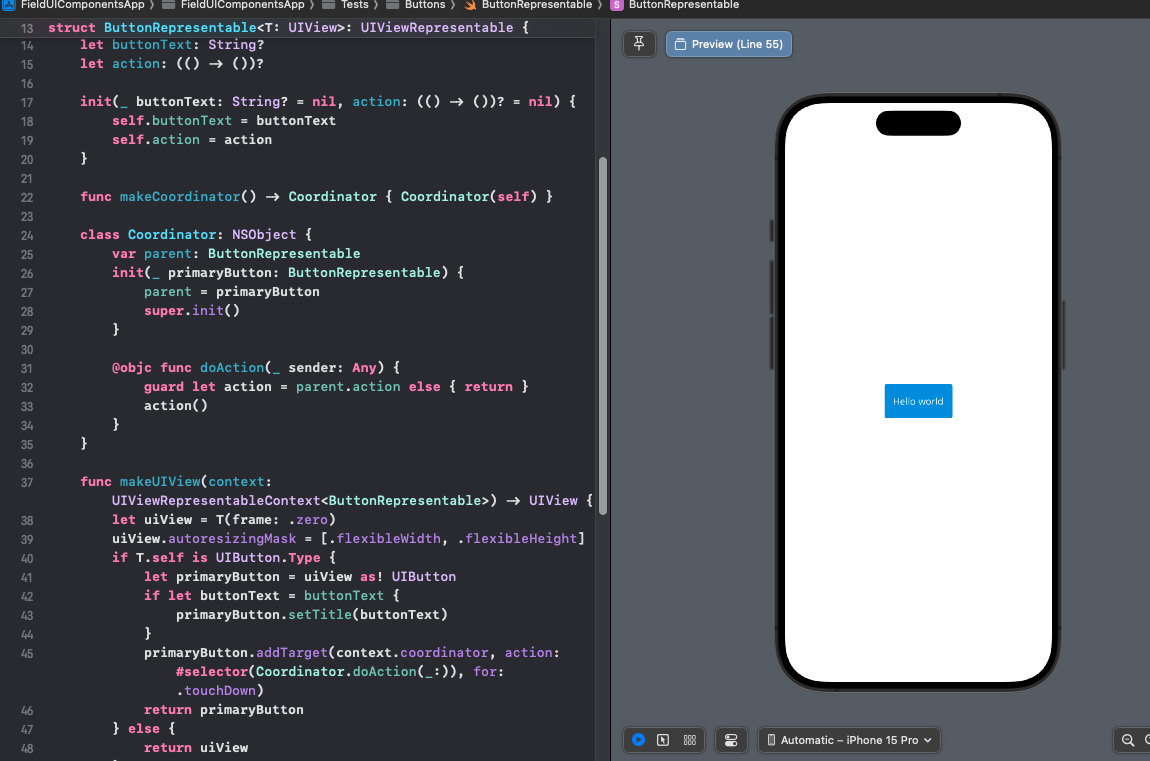
\includegraphics[width=1\textwidth]{Images/iOSButtonRepresentable.png}
    \caption{ButtonViewRepresentable failas}
    \label{fig:buttonViewRepresentable}
\end{figure}

\newpage
\subsubsection{Custom Toast message on Android}
Ši užduotis buvo skirta realizuoti UX sukurtą iššokančių žinučių (\emph{angl. Toast messages}) komponentą Android ir iOS operacinėse sistemose. 
Buvo sukurti FieldUIComponents app langai, kuriuose galima įvairiais būdais ištestuoti iššokančias žinutes.

Pasirinkau atlikti šią užduotį Android prietaisuose. 

Reikalavimai atliekant užduotį:
\begin{enumerate}
    \item Sukurti padengtą testais FieldUIComponents komponentą.
    \item Sukurti naują iššokančių žinučių komponentą.
    \begin{enumerate}
        \item Teksto žinutė
        \begin{enumerate}
            \item Tekstas turi tilpti į vieną eilutę.
            \item Jei tekstas užima daugiau vietos, sutrumpinti su \enquote{...}.
            \item Komponento animacija turi kiek galima daugiau sutapti su maketo animacijomis.
        \end{enumerate}
        \item Iššokančios žinutės animacijos trukmė - 3 sekundės.
        \item Iššokanti žinutė galima paslėpti paspaudus ant jos ar atlikus tempimo į viršų gestą.
    \end{enumerate}
    \item Iššokančių žinučių eilė:
    \begin{enumerate}
        \item Iššokančios žinutės patenka į eilę, rodomos viena po kitos, paslepiamos tokia pačia tvarka kaip ir buvo parodytos.
        \item Tokios pačios žinutės nerodomos 2 kartus.
    \end{enumerate}
\end{enumerate}
\newpage
Iš pradžių buvo sukurtas iššokančios žinutės komponentas (\ref{fig:pill} paveikslėlis). Komponentui pritaikytos gestų atpažinimo, paspaudimo funkcionalumas, teksto sutrumpinimas (\ref{fig:pillCode} paveikslėlis).

\begin{figure}[htbp!]
    \centering
    \begin{minted}[linenos,tabsize=1,breaklines]{kotlin}
@Composable
fun Pill(
    modifier: Modifier = Modifier,
    text: String,
    fontSize: TextUnit = dimensionResource(id = R.dimen.toast_font_size).value.sp,
    horizontalPadding: Dp = dimensionResource(id = R.dimen.toast_padding_horizontal),
    verticalPadding: Dp = dimensionResource(id = R.dimen.toast_padding_vertical)
) {
    Surface(
        modifier = modifier
            .padding(horizontal = horizontalPadding),
        shape = CircleShape,
        color = colorResource(R.color.toastBackground)
    ) {
        Row(
            modifier = Modifier
                .wrapContentWidth()
                .padding(horizontalPadding, verticalPadding),
            horizontalArrangement = Arrangement.Center
        ) {
            Text(
                text = text,
                textAlign = TextAlign.Center,
                fontSize = fontSize,
                color = Color.White,
                style = MaterialTheme.typography.body2,
                maxLines = 1,
                overflow = TextOverflow.Ellipsis
            )
        }
    }
}
    \end{minted}
    \caption{Iššokančios žinutės komponento kodas}
    \label{fig:pillCode}
\end{figure}
\newpage
Sukurtas \enquote{ToastViewModel}, kuris rūpinasi iššokančių žinučių eile, patikrina eilėje esančias žinutes, jei eilėje egzistuoja žinutė, antrą kartą jos neparodys (\ref{fig:ToastViewModel} paveikslėlis). Taip pat galima pateikti žinutės trukmę. pasibaigus trukmei, žinutė išmetama iš eilės.

\begin{figure}[htbp!]
    \centering
    \begin{minted}[linenos,tabsize=1,breaklines]{kotlin}
class ToastViewModel : ViewModel() {
    private val _toastDataState = MutableStateFlow<ToastData?>(null)
    val toastDataState = _toastDataState.asStateFlow()

    private val mutex = Mutex()

    private var pendingMessages: MutableSet<String> = mutableSetOf()

    fun showToast(
        message: String,
        duration: Long = 3000L
    ) {
        if (pendingMessages.isEmpty() || pendingMessages.last() != message) {
            pendingMessages.add(message)
            viewModelScope.launchSafe {
                mutex.withLock {
                    try {
                        return@launchSafe suspendCancellableCoroutine { continuation ->
                            _toastDataState.value = ToastData(message, duration, continuation)
                        }
                    } finally {
                        _toastDataState.value = null
                        pendingMessages.remove(message)
                    }
                }
            }
        }
    }
}
    \end{minted}
    \caption{ToastViewModel programinis kodas}
    \label{fig:ToastViewModel}
\end{figure}

\newpage
Buvo sukurtas \enquote{ToastHost}, skirtas tvarkingai, su animacijomis parodyti iššokančias žinutes  (\ref{fig:ToastHost} paveikslėlis). Panaudota 1,5 konstanta, kad paslėpti iššokančią žinutę, kai kyla į viršų už navigacijos juostos. Standumo ir kiti animacijos parametrai parinkti, kad kuo labiau atitiktų Figma maketų animacijas.

\begin{figure}[htbp!]
    \centering
    \begin{minted}[linenos,tabsize=1,breaklines]{kotlin}
...
val animationOffset: (Int) -> Int = { (heightToDropPx + it * 1.5).toInt() * -1 }
val springAnimationSpec: FiniteAnimationSpec<IntOffset> = spring(
    dampingRatio = Spring.DampingRatioMediumBouncy,
    stiffness = Spring.StiffnessMedium
)

LaunchedEffect(currentToastData) {
    setVisibility(true)
    delay(currentToastData.duration)
    setVisibility(false)
}

AnimatedVisibility(
    modifier = modifier.padding(top = heightToDrop),
    enter = slideInVertically(springAnimationSpec, initialOffsetY = animationOffset),
    exit = slideOutVertically(springAnimationSpec, targetOffsetY = animationOffset),
    visibleState = isVisible,
    content = { toast() }
)
...
    \end{minted}
    \caption{ToastHost programinis kodas}
    \label{fig:ToastHost}
\end{figure}

\newpage
Kadangi \enquote{Jetpack Compose} komponentų tiesiogiai integruoti į fragmentais pagrįstą programėlę, reikėjo sukurti papildomą klasę \enquote{Toasts} (\ref{fig:Toasts} paveikslėlis). Jame padavus tėvinį vaizdą (\emph{angl. root view}) programiniu būdu prideda \enquote{Jetpack Compose} komponentą. Kadangi programėlė yra suprogramuota naudojantis daug fragmentų ir 1 \textit{activity}, iššokančios žinutės matysis visoje programėlėje. Galutinį rezultatą galima matyti \ref{fig:modelToastView} paveikslėlyje.

\begin{figure}[htbp!]
    \centering
    \begin{minted}[linenos,tabsize=1,breaklines]{kotlin}
class Toasts(private val context: Context) {
    private var view: View? = null
    fun addToastView(activityRootLayout: ViewGroup?) {
        val rootView = activityRootLayout ?: return
        if (view == null)
            createToastView(rootView)
    }

    private fun createToastView(rootView: ViewGroup) {
        val view = ComposeView(context).apply {
        setViewCompositionStrategy(ViewCompositionStrategy.DisposeOnViewTreeLifecycleDestroyed)
            setContent {
                Column {
                    Toast(toastViewModel = toastViewModel)
                }
            }
        }

        this.view = view
        rootView.addView(view)
        rootView.bringChildToFront(view)
        view.requestLayout()
    }
}
\end{minted}
    \caption{Toasts komponentas}
    \label{fig:Toasts}
\end{figure}
\newpage

\subsection{Praktikos metu naudotos technologijos}
Šiame poskyryje aprašomos technologijos, kurias naudojau praktikos metu ir pavyzdžiai, kur jos buvo naudojamos. 
Atlikdamas praktiką mobiliųjų įrenginių kūrimo komandoje turėjau galimybę dirbti su įvairiomis pripažintomis ir naujausiomis technologijomis. Toliau aprašoma pagrindinių \enquote{Android} ir \enquote{iOS} technologijų, kuriomis naudojausi, apžvalga:

Jetpack Compose yra modernus Google vartotojo sąsajų priemonių rinkinys, skirtas Android taikomųjų programų vartotojo sąsajoms kurti. Jame naudojamas deklaratyvusis metodas, kai kūrėjai aprašo norimą naudotojo sąsajos būseną, o ne tai, kaip ją pasiekti žingsnis po žingsnio. Taikant šį požiūrį kodas gali būti glaustesnis ir lengviau suprantamas.  "Jetpack Compose" naudoja "Kotlin" galimybes, todėl kūrėjai gali kurti vartotojo sąsajos komponentus kaip funkcijas.  Tai gali pagerinti kodo skaitomumą ir palaikymą.


\subsubsection{Kotlin}
Kotlin yra viena iš populiariausių programavimo kalbų kuriant Android mobiliąsias programėles. Lyginant su Java programavimo kalba, Kotlin yra modernesnė, null reikšmių saugumu. Kotlin lengvai pritaikoma senesniuose projektuose, parašytuose su Java ir XML vartotojo sąsaja, paprasta atnaujinti seną kodo bazę. Sintaksės panašumas į kitas programavimo kalbas, padeda lengvai ir greita išmokti Kotlin programavimo kalbos pagrindus.
Visos praktikos metu Kotlin programavimo kalbą naudojau kurti naudotojo sąsajos logiką, tvarkyti duomenis ir integruoti naujus komponentus į turimą mobiliąją programėlę.

\subsubsection{Jetpack Compose}

"Jetpack Compose" yra Android rekomenduojamas modernus įrankių rinkinys, skirtas vietinei vartotojo sąsajai kurti. Rinkinys supaprastina ir pagreitina Android mobiliųjų programėlių vartotojo sąsajos kūrimą. Jame taikomas deklaratyvus metodas,

% % \begin{figure}
% %     \centering
% %     \begin{minted}[linenos,tabsize=1,breaklines]{kotlin}
% %     @Composable
% %     fun TestListParameterView(
% %         values: List<String>,
% %         initialMessage: String = "Initial message",
% %         labelText: String = "Label",
% %         onRemove: (String) -> Unit,
% %         onAdd: (String) -> Unit
% %     ) {
% %         var text by rememberSaveable { mutableStateOf(initialMessage) }
% %         Column {
% %             LazyColumn(modifier = Modifier.height(200.dp)) {
% %                 items(items = values) { value ->
% %                     Row {
% %                         Text(
% %                             modifier = Modifier.height(44.dp).fillMaxWidth(0.9f),
% %                             maxLines = 2,
% %                             style = MaterialTheme.typography.body2,
% %                             text = value,
% %                             overflow = TextOverflow.Ellipsis
% %                         )
% %                         Spacer(modifier = Modifier.weight(1f))
% %                         TextButton(
% %                             modifier = Modifier.width(44.dp).background(Color.Transparent),
% %                             onClick = { onRemove(value) },
% %                             content = { Icon(painter = painterResource(...)) }
% %                         )
% %                     }
% %                 }
% %             }
% %             OutlinedTextField(
% %                 modifier = Modifier.fillMaxWidth(),
% %                 value = text,
% %                 onValueChange = { text = it },
% %                 label = { Text(labelText) }
% %             )
% %             Button(onClick = {
% %                 if (text.isNotBlank()) {
% %                     onAdd(text)
% %                     text = ""
% %                 }
% %             }) { Text(text = "Add") }
% %         }
% %     }
% %     \end{minted}
% %     \caption{Jetpack Compose programinis kodas}
% %     \label{fig:composeCode}
% % \end{figure}

% % \begin{figure}[htbp!]
% %   \centering
% %   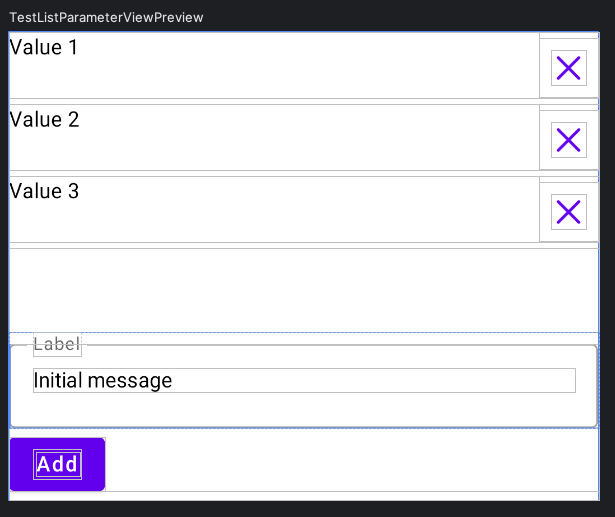
\includegraphics[width=0.8\linewidth]{Images/JetpackCompose.png}
% %   \caption{Jetpack Compose komponento peržiūra}
% %   \label{fig:example}
% % \end{figure}


\subsubsection{Swift}
Swift yra galinga, tačiau nesunki pradedantiesiems programavimo kalba, kurią Apple sukūrė savo įrenginiams. Lyginant su \enquote{Objective-C}, Swift pasižymi švariu ir glaustu stiliumi, artimesniu natūraliai kalbai. Priešingai nei \enquote{Objective-C}, Swift atlieka daugiau automatinio atminties valdymo ir tipų tikrinimo, tai padeda išvengti gedimų ir klaidų, kurios dažniau pasitaiko \enquote{Objective-C} kalboje. Dėl šių priežasčių, dėmesio, programinį kodą  greita parašyti ir lengva prižiūrėti. Nors \enquote{Objective-C} dar naudojama esamuose projektuose, integruoti Swift nesunku net ir į itin senus projektus. Su Swift programavimo kalba galima rašyti programėles iPhone, iPad, MacBook, Apple watch įrenginiams. Neseniai atsiradusiam \enquote{Apple vision pro} prietaisui irgi yra galimybė kurti programas šia programavimo kalba. 

\subsubsection{SwiftUI}

\enquote{SwiftUI} - tai naujas Apple karkasas įrenginių naudotojo sąsajų kūrimui. Skirtingai nuo storyboards sąsajų kūrimo, kuris remiasi vizualiniu komponentų dėliojimu ekrane, \enquote{SwiftUI} naudoja deklaratyvų požiūrį. Storyboards vartotojo sąsajos konvertuojamos į XML,  kas yra gana nepatogu, kai atliekamos programinio kodo pakeitimų peržiūros. Kaip ir \enquote{Jetpack compose}, \enquote{SwiftUI}, kode galima atlikti vartotojo sąsajos būsenų valdymą, deklaratyviai konstruoti vartotojo sąsają. Išbandžius abi technologijas iOS vartotojo sąsajos kūrimo technologijas, norint suprasti ir atlikti kodo pakeitimus esamame projekte, \enquote{SwiftUI} yra geresnis programavimo karkasas, suprasti kodo veikimo principus, prireiks mažiau laiko.

\section{Rezultatai, išvados ir pasiūlymai}

\textbf{Praktikos darbo privalumai}:
\begin{enumerate}
    \item Taikomos naujos technologijos.
    \item Galimybė laisvai rinktis norimas užduotis.
    \item Draugiška, padedanti komanda.
\end{enumerate}
\bigskip

\textbf{Praktikos darbo trūkumai}:
\begin{enumerate}
    \item Praktikantai dažnai jaučiasi izoliuoti vienoje komandoje, baugu susipažinti su kitais praktikantais, praktikantų susitikimai nuotoliniai, kas pasunkina socializacijos aspektą.
\end{enumerate}
\bigskip

\textbf{Įgytos žinios ir patirtis praktikos metu:}
\begin{enumerate}
    \item Įgyta patirties rašant programinį kodą Kotlin programavimo kalba.
    \item Įgyta žinių apie “Jetpack Compose” Android įrankių rinkiniu skirtu kurti vartotojo sąsają.
    \item Lavinau darbo komandoje gebėjimus ir darbo "Kanban" projektų valdymo metodo pagalba.
    \item Įgyta patirties rašant kodą su švaraus ir kokybiško rašymo principais ir geriausiomis praktikomis. 
    \item Įgyvendintas naujas funkcionalumas Android programėlėje.
\end{enumerate}
\bigskip

\textbf{Pasiūlymai įmonei}:
\begin{enumerate}
    \item Įmonėje, šiuo metu, į praktikos pozicijas primami tik programuotojai ir testuotojai. Būtų galima išplėsti praktikos pozicijų pasirinkimą, pridedant projektų vadovo, vartotojo sąsajos dizainerių pozicijas.
    \item Atliekant praktiką, neteko susidurti su realių programinės įrangos, funkcionalumų įvertinimo iš vartotojų pusės. Bet 2 mėnesiai, manau, yra per mažas laiko tarpas, kad įgyvendintas funkcionalumas pasiektų vartotojus.
    \item Pirmą kartą pamačius projektą, buvo nelabai aišku, koks jo pilnas funkcionalumas, didžiąją dalį funkcionalumo atradau atliekant programinio kodo pakeitimus. Galima praktikantams, prieš pradedant rašyti kodą, pristatyti projekto funkcionalumą.
\end{enumerate}
% \begin{enumerate}
%     % \item Grupinių projektinių darbų pristatymų metu per daug skiriama dėmesio sistemos funkcionalumui ir pristatymo sklandumui. Dėl to dažniausiai nukenčia sistemos testavimas -- jaunieji programuotojai nerašo testų, kadangi tai nėra vertinama pristatymo metu.
% \end{enumerate}


\textbf{Pasiūlymai universitetui}
\begin{enumerate}
    \item Praktikos metu teko dirbti prie mobiliųjų programėlių, jų funkcionalumo tobulinimo, universitete, mano žiniomis, privalomojo ar pasirenkamojo dalyko programų sistemų programoje nėra, tad būtų pravartu turėti bent vieną kursą, kuris leistų susipažinti ne tik su interneto svetainių kūrimu, bet ir su kitokia programų kūrimo paradigma.
    \item Galimybė dirbti prie žymiai didesnio projekto. Paskaitų metu, dažniausiai dirbama prie nuo nulio kuriamų projektų, tačiau darbas prie didelės kodo bazės, kurios ankščiau studentas nematė, būtų naudinga patirtis, nes atėjus į darbovietę, studentas, dažniausiai negaus kurti projekto nuo nulio ir teks dirbti prie senesnio, ne su visomis geriausiomis programavimo praktikomis.
    \item Pridėti vartotojo sąsajos testavimo modulį. Universitete testavimo kurse, buvo kalbama apie vienetinius, integracinius, prasiskverbimo testus, apie vartoto sąsają nebuvo užsiminta. Būtų galima supažindinti studentus su pagrindiniais mobiliųjų programėlių testavimo būdais, nes didžiąją dalį vartotojo sąsajos testavimo žinių įgavau tik praktikos metu. 
\end{enumerate}

\newpage

\section{Priedai}
\begin{figure}[htbp!]
    \centering
    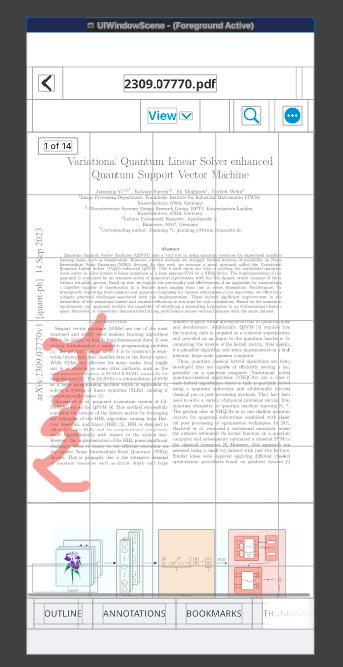
\includegraphics[width=0.5\textwidth]{Images/PdfTronViewController.png}
    \caption{PdfTronViewController ekranas}
    \label{fig:pdfViewController screen}
\end{figure}

\begin{figure}[htbp!]
    \centering
    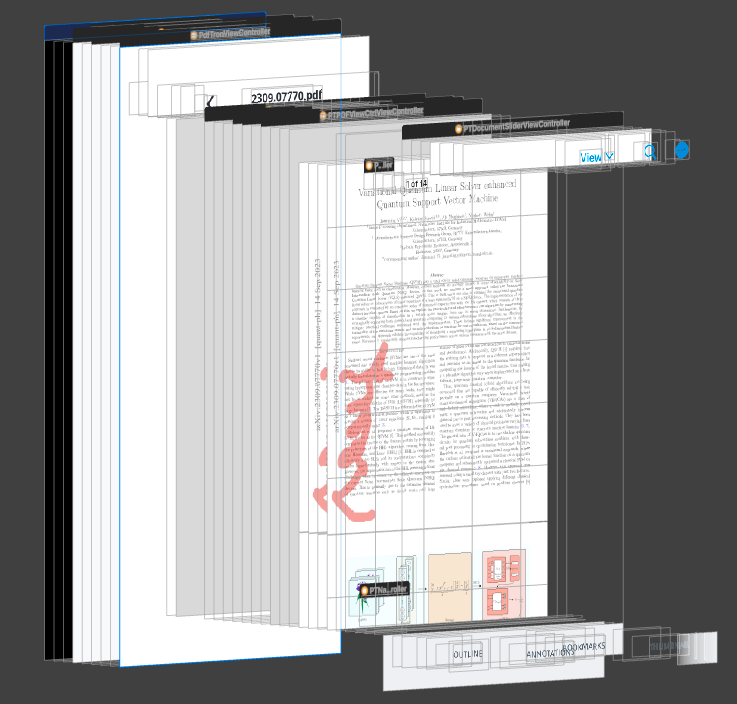
\includegraphics[width=0.8\textwidth]{Images/SideViewPdfViewController.png}
    \caption{PdfTronViewController dekompozicija}
    \label{img:pdfViewController}
\end{figure}

\begin{figure}[htbp!]
    \centering
    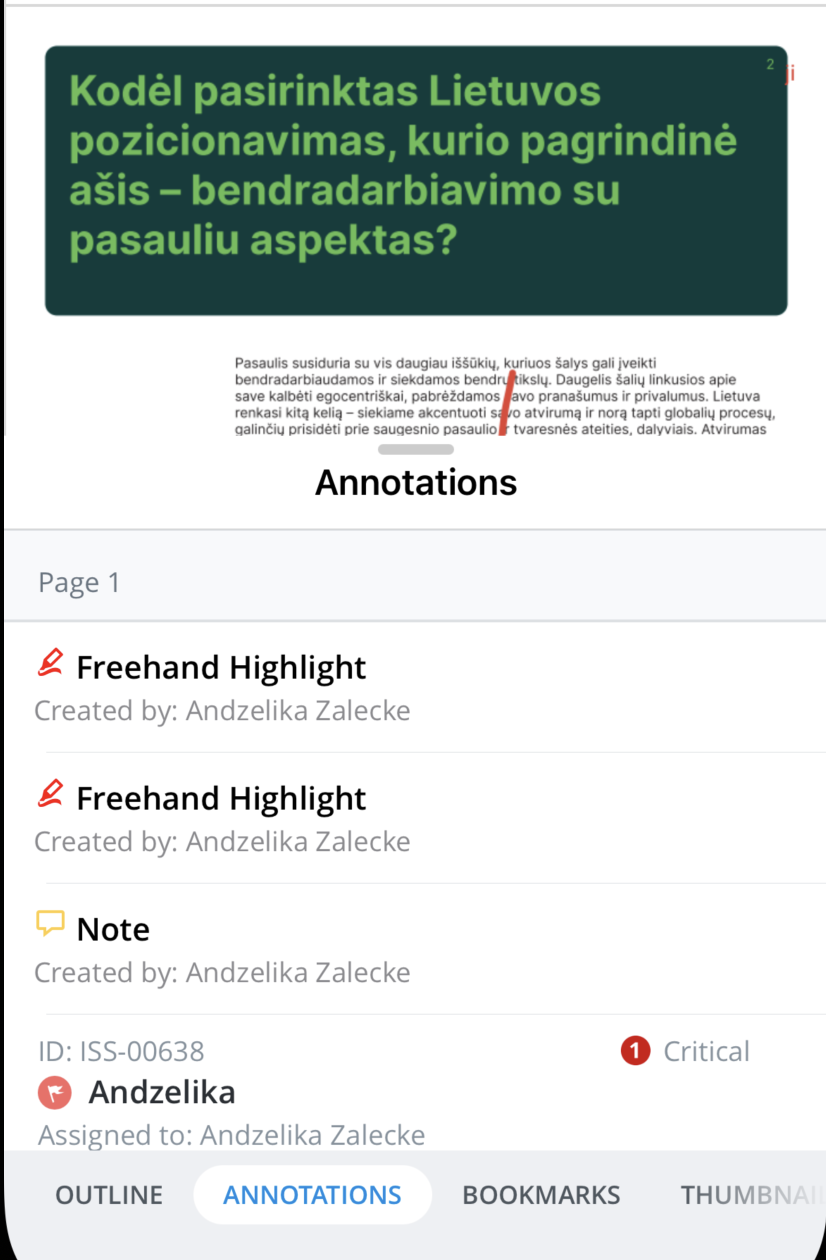
\includegraphics[width=0.6\textwidth]{Images/annotationList.png}
    \caption{Anotacijų sąrašo komponentas}
    \label{img:annotationList}
\end{figure}

\begin{figure}[htbp!]
    \centering
    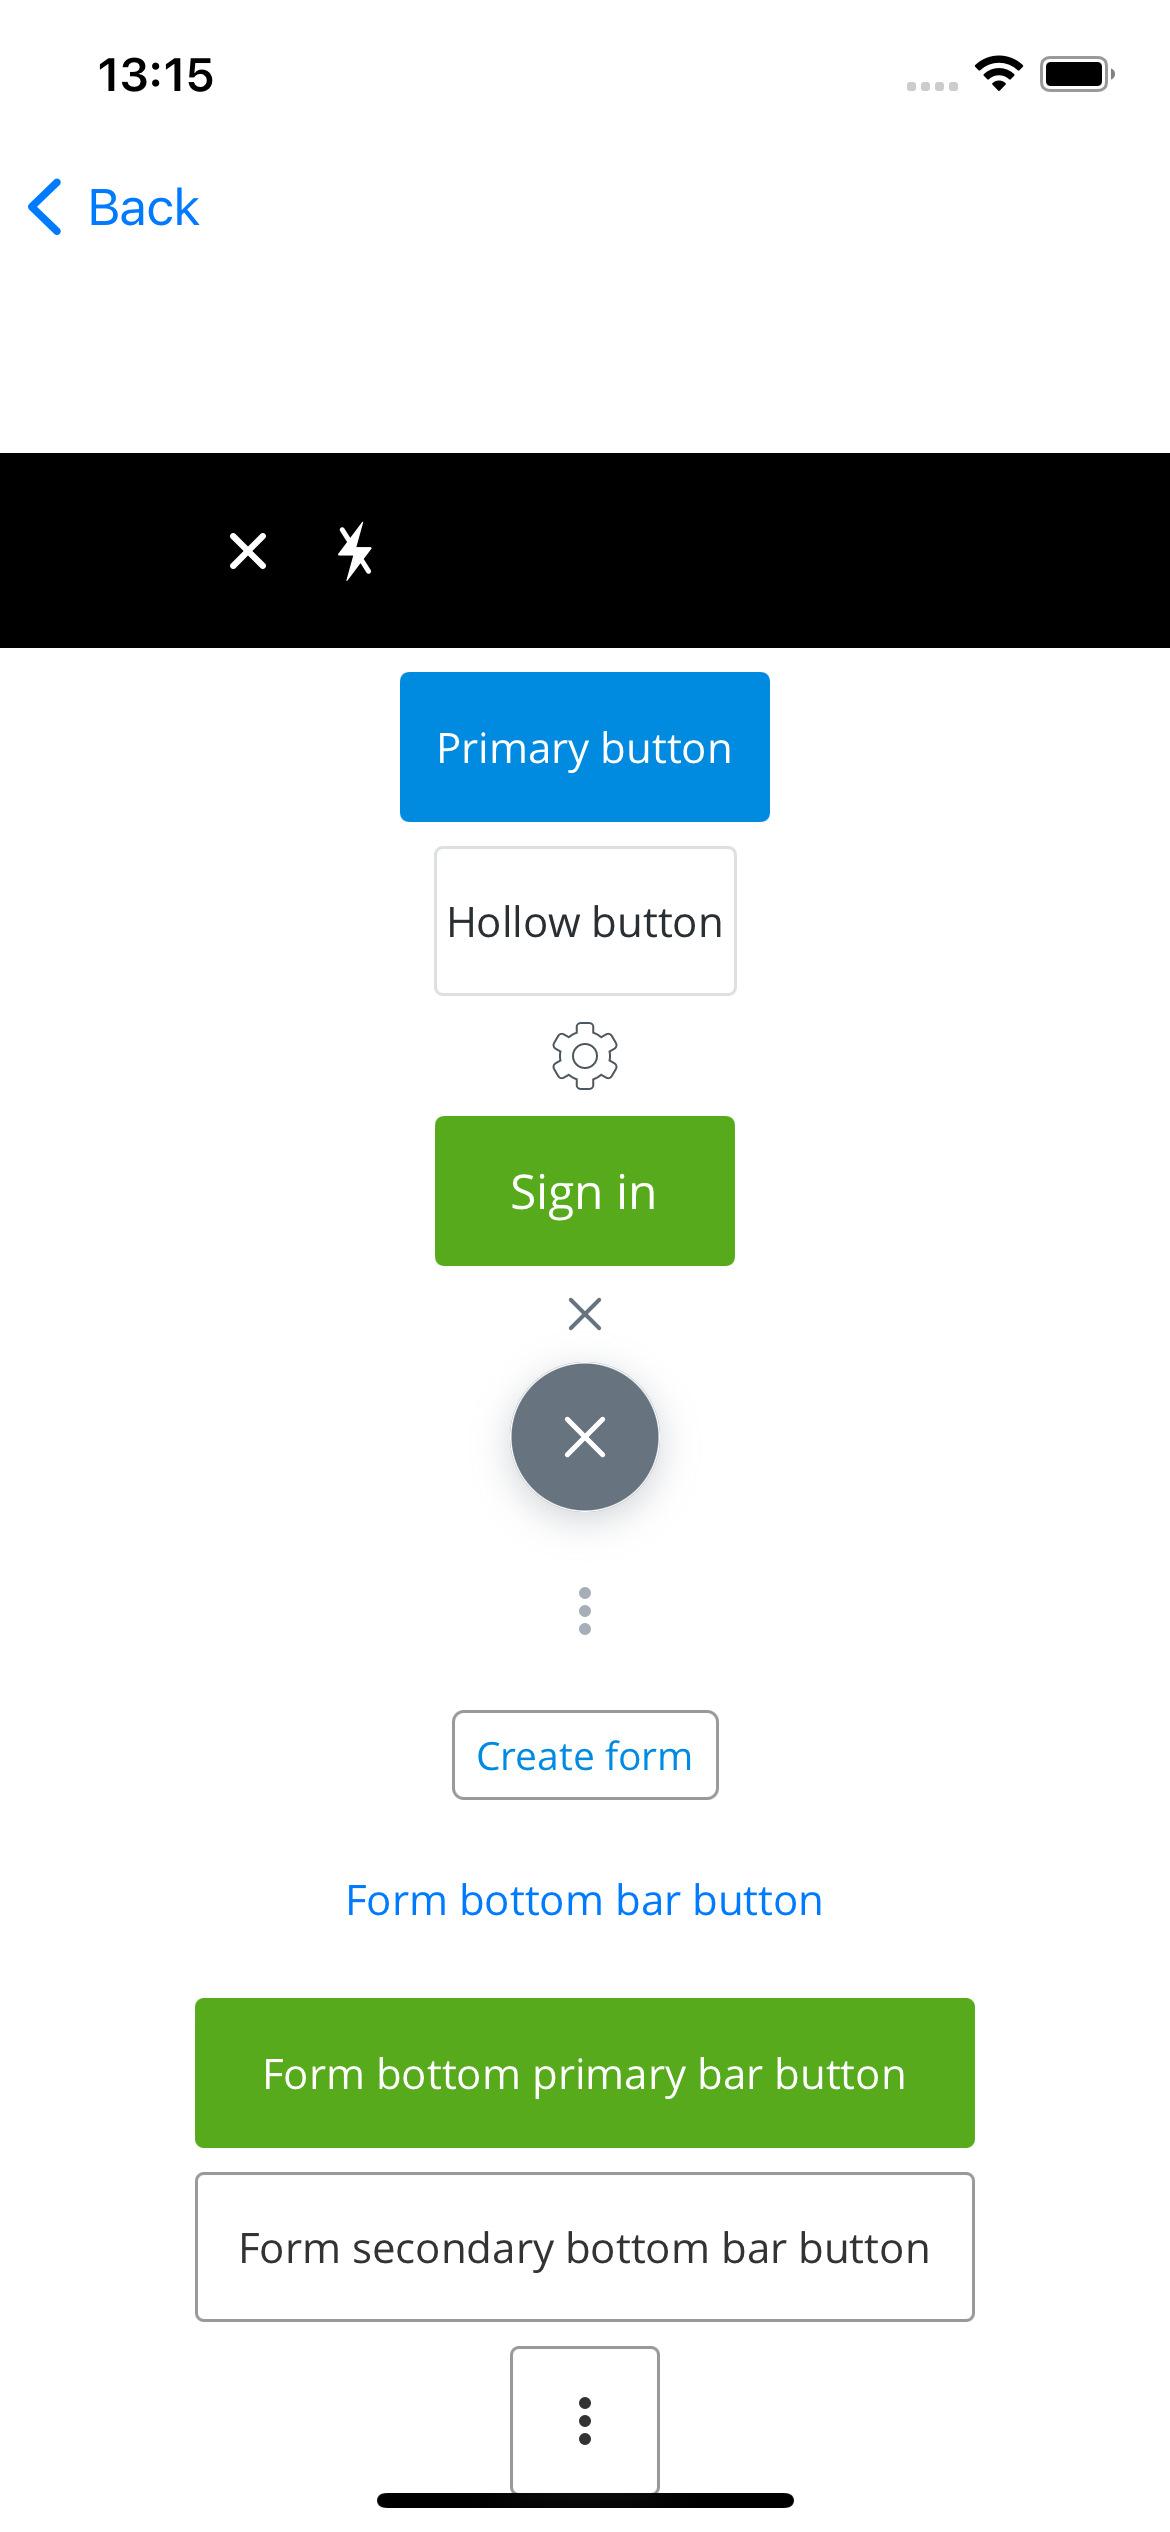
\includegraphics[width=0.6\textwidth]{Images/buttonsView.png}
    \caption{Projekto mygtukų langas}
    \label{fig:buttonsView.png}
\end{figure}

\begin{figure}[htbp!]
    \centering
    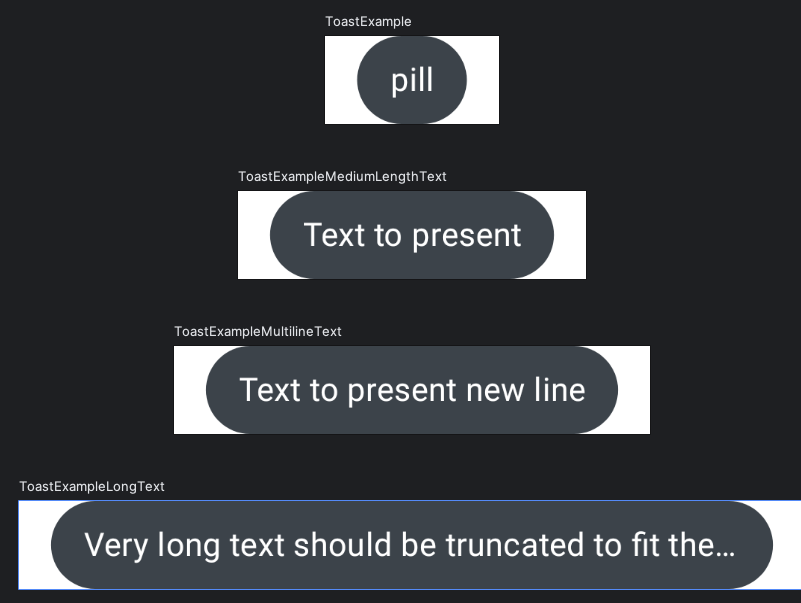
\includegraphics[width=0.7\textwidth]{Images/pillAndroid.png}
    \caption{Iššokančios žinutės komponentas}
    \label{fig:pill}
\end{figure}

\begin{figure}[htbp!]
    \centering
    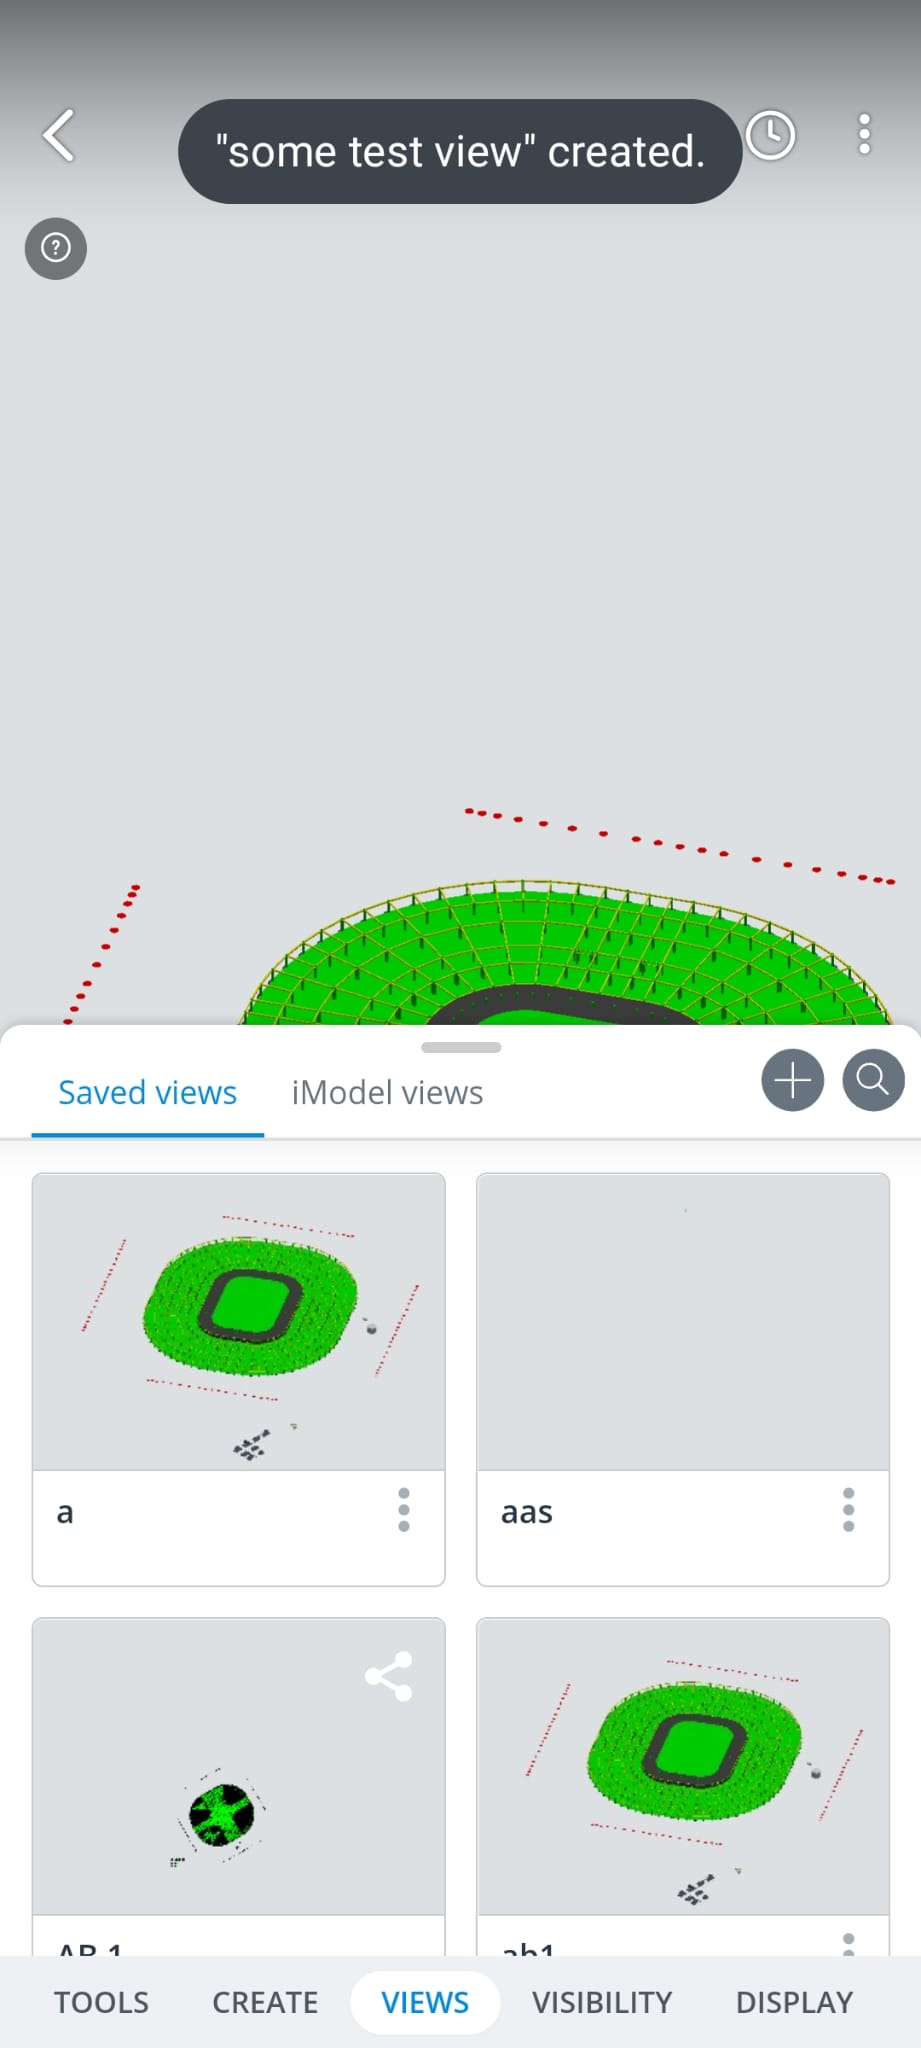
\includegraphics[width=0.5\textwidth]{Images/toastView.jpeg}
    \caption{Iššokančios žinutės komponento pavyzdys programėlėje}
    \label{fig:modelToastView}
\end{figure}
\end{document}

